
\section{Jets}


\begin{figure}[t]
 \centering
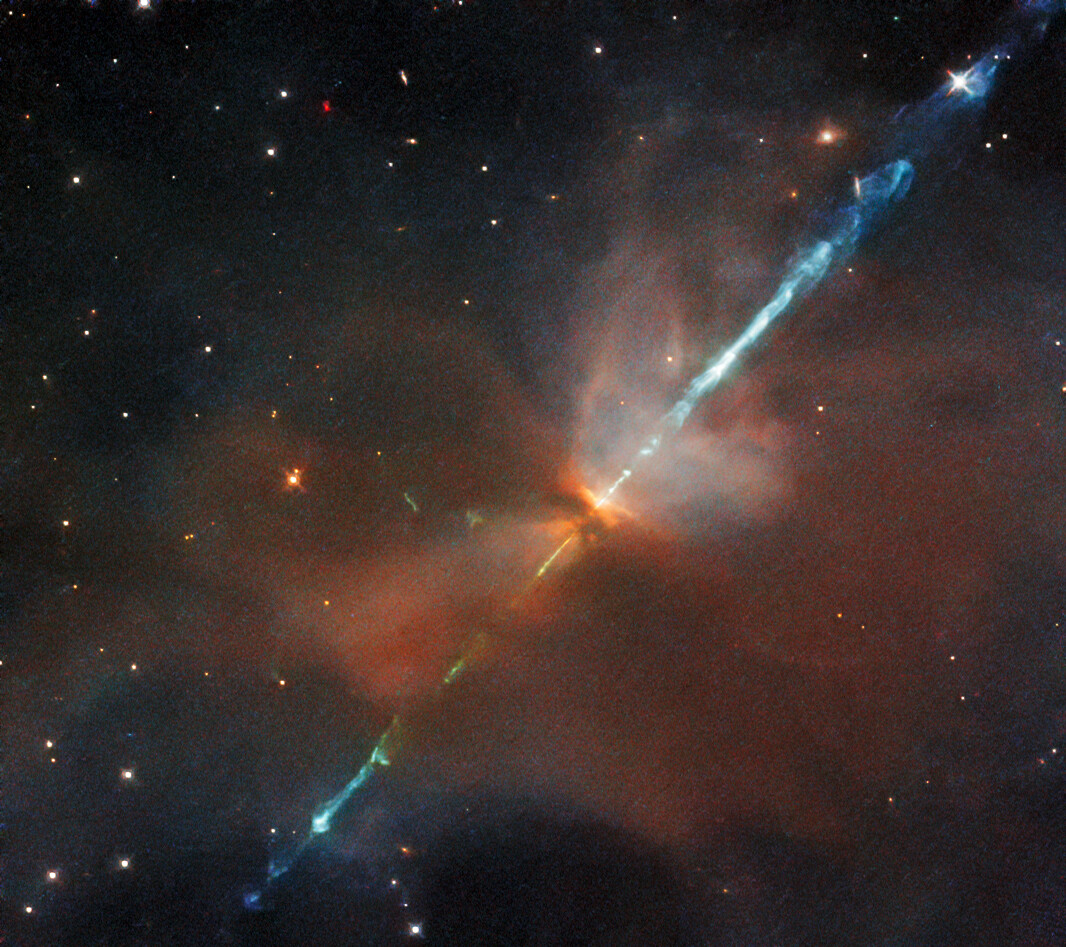
\includegraphics[width=6cm]{figs/HH111_-_HST_-_Potw2135a.jpg}
\caption{HST composite image of HH~111. Image credit: ESA/Hubble \& NASA, B. Nisini. \label{fig:HH111} }
\end{figure}


% https://en.wikipedia.org/wiki/File:HH111_-_HST_-_Potw2135a.jpg

Protostellar outflows  were ``discovered''\footnote{The nebulosity around T~Tau was first described in the 19th century  by \citet{Burnham_1890, Burnham_1894}.} by \citet{Herbig_1950,Herbig_1951} and \citet{Haro_1952,Haro_1953} in the early 1950s. These authors studied the optical, nebular emission around young stars. This ``nebular'' emission from forbidden emission lines (FELs) is typically concentrated in individual, relatively distinct emission regions along a relatively straight path extending away from a young star (see Fig.~\ref{fig:HH111}). These emission knots  are called Herbig-Haro (HH) objects and trace plasma ejected from a young stellar system, which then propagates in the ambient medium with supersonic velocities. Outflows in pre-main sequence stars (PMS) are detected in a wide range of wavelengths and show very different morphologies, from jets with opening angles of only a few degree to less-collimated, wide-angle outflows. 
They are seen as long as the central star is accreting, and the ratio between outflow to accretion mass rates of roughly $\dot{M}_{out}/\dot{M_{acc}}\sim0.1$ appears constant throughout this phase \citep[e.g.,][]{Cabrit_2007, Nisini_2018}. Because the accretion rate decreases with time, the mass-loss rate through the outflow also decreases with time. However, the current picture is that the jet physics remain the same during the entire accretion phase.

Protostellar outflows are powered by a variety of mass ejection phenomena occurring during the star formation process, which are intimately related to the accretion process. 
Most outflow observations are compatible with magneto-centrifugally launched disk winds from the inner regions of protoplanetary disks \citep[roughly 0.1\,au to 10\,au, see][]{Frank_2014}. However, there are other possible launch regions, too. First, stellar winds can launch from the hot stellar corona much like the solar wind \citep{Matt_2005}. In analogy with the solar wind, such stellar winds are very hot ($\gtrsim10^6$\,K) and may cool via X-ray emission. Second, magnetospheric ejections can launch from the region between the star and the inner edge of the disk \citep{Zanni_2013}. Third, X-winds could be launched from a narrow region close to the inner edge of the disk \citep{Shu_1994}. Even more mechanisms to launch outflows may exist  in the young, class~0 objects, but they produce slower outflow velocities and are therefore not related to the observed X-ray emission and ignored here.

Protostellar jets are typically studied in FELs, because shocks within the outflow heat the plasma to temperatures of roughly $10^4\,$K. According to Eq.~\ref{eqn:Tshock}, such a post shock temperature corresponds to shock velocities of $\sim20-30$\,km\,s$^{-1}$.
%
Because of the low densities ($\lesssim10^4\,$cm$^{-3}$ beyond few tens of au), radiative cooling of the shock heated plasma is dominated by hydrogen (e.g., H$\alpha$) and metallic FELs such as [O~{\sc i}], [S~{\sc ii}], and [Fe~{\sc ii}].
Nevertheless, protostellar jets have been studied from radio over (near-) IR to optical and UV wavelengths.
However, there were no indications for plasma temperatures of $T\gg10^5\,$K. Hence, the detection of protostellar jets in X-rays came to a surprise.

% These lines (or line ratios) allow one to estimate the physical properties of the emitting plasma \citep[temperature, density, ionization degree, e.g., ][]{Bacciotti_1999}.
% 
% 
% 
% {\color{red} TBD: Magnetic towers \citep{Huarte_2012}? }
% 
% {\color{red} Reverse shock!}

\subsection{X-rays from protostellar jets}

\begin{figure}[t]
\centering

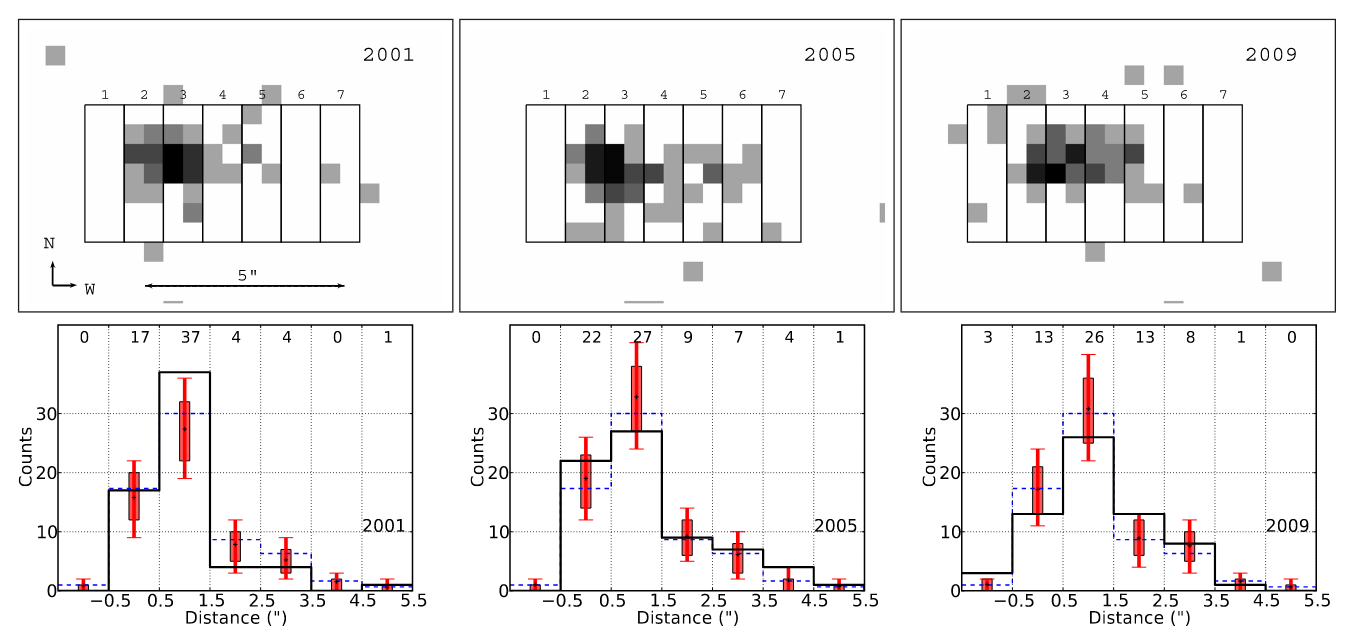
\includegraphics[height=6cm]{figs/hh154}
% % %
\caption{Evolution of the X-ray emission from HH 154. From \citet{Schneider_2011}. \label{fig:hh154} {\color{red} color version of the figure for the top panels?}}
\end{figure}


% \subsection{X-ray jet observations}
The first X-ray detections of protostellar jets were obtained almost simultaneously in 2001 by \citet{Pravdo_2001} using Chandra (HH~2) and \citet{Favata_2002}
using XMM-Newton (HH~154 or L\,1551~IRS\,5, see Fig.~\ref{fig:hh154}), both launched from class~I objects. The association of the Chandra detected X-ray emission to HH~2 is straight forward, because the X-ray emission  (a) spatially coincides with one of the optically brightest knots, (b) appears extended, and (c) the X-ray spectrum is soft ($T\sim1.2\times10^6\,$K) unlike typical coronae of young stars. In contrast, the association of the X-rays from the L\,1551~IRS\,5 complex to HH~154 strongly builds on the severe extinction towards the protostellar sources while the jet suffers much less extinction \citep[$A_V(jet)\sim10\,$mag vs $A_V(protostars)\gtrsim150$\,mag, e.g.,][]{White_2000,Fridlund_2005}. This high $A_V$ towards the stellar sources led \citet{Favata_2002} to ascribe the X-rays to HH~154 despite the proximity of the X-ray emission to the stellar position and the comparably high mean X-ray energies ($\sim1\,$keV), simply because any reasonable X-ray emission from the stellar system would not make it directly to the observer. Later, \citet{Bally_2003}, located the X-rays from HH~154 to the base of the outflow using new Chandra data; the location of the X-rays may be in a region where the outflow is collimated to the narrow jet observed further away from the sources. 

These two early discoveries of X-ray emission  from protostellar jets already indicate two different phenomena, namely emission from the jet base and from working surfaces at large distances to the driving sources, i.e., from individual jet knots. To simplify the discussion, we separate these two phenomena here, because they may represent tracers of different mechanisms.


\subsubsection{X-rays from jet knots}

We start our discussion with the X-ray emission from jet knots at distances well beyond the jet collimation region and the protostellar envelope ($d\gg100\,$au, i.e., $\gg1$ arcsec for the nearest jets), because this allows us to derive the physical requirements to produce significant X-ray emission within outflows. Examples of this sub-class of X-ray emitting jets are HH~2 \citep{Pravdo_2001}, HH~80/81 \citep{Pravdo_2004}, TKH~8 \citep{Tsujimoto_2004}, the jet from HD~163296 \citep[HH~409][]{Swartz_2005,Guenther_2013},   HH 168 \citep{Pravdo_2005,Schneider_2009}, HH~210 \citep{Grosso_2006}, HH~216 \citep{Linsky_2007}, Z CMa \citep{Stelzer_2009}, and possibly, HH~248 \citep{Lopez_2015}; the driving sources range from low to high mass objects suggesting that 
the source details do not dominate the jet's appearance in X-rays. However, the relatively high fraction of high-mass objects driving X-ray emitting jets may indicate that their jets more frequently favor X-ray emission. 


The jet's X-ray emission is typically seen close to emission at other wavelengths from cooler plasma   \citep[$T\sim10^4$\,K, e.g.,][]{Pravdo_2004,Grosso_2006,Schneider_2012}.  In some cases, the X-ray emitting knots have been reported to also show [O~{\sc iii}] emission \citep[$T\sim10^5$\,K, see ][]{Grosso_2006}  and the X-ray emitting knots tend to be among the fastest knots with space velocities of $\gtrsim400$\,km\,s$^{-1}$ \citep[e.g.,][]{Pravdo_2001} while the slower knots of the same jets do not show up in X-rays. The X-ray emission in HH~2  moves along the jet path with high velocity \citep{Schneider_2012} so that shocks are thought to be the most likely explanation for the X-ray emission although the X-rays may not come from the leading working surface in all cases, but are rather displaced somewhat towards the driving sources \citep[][]{Pravdo_2005}.

A key requirement to produce significant X-ray emission from shocks is a sufficiently high flow velocity so that the post-shock plasma is high enough to emit significantly in the X-ray range. The derived temperatures for the X-ray emitting plasma are roughly  in the low to medium MK range so that shock velocities $v_{shock}$ of $500\pm200$\,km\,s$^{-1}$ are required (the physics of shock heating is the same as in the accretion shock, see ~Eq.~\ref{eqn:Tshock}). Such shock velocities may result where the jet flow encounters low velocity  material in front of it, either from previous ejecta or dense clumps in the molecular cloud. Based on proper motion measurements \citep{Eisloffel_1994}, \citet{Schneider_2012} suggest that the X-ray emitting knot in HH~2 was formed by the interaction of a fast (490\,km\,s$^{-1}$) knot overtaking a slower one (220\,km\,s$^{-1}$) resulting in shock and post shock velocities compatible with the measured values.



The second requirement is a sufficient X-ray luminosity. The observed X-ray luminosities range from a few $10^{29}$\,erg\,s$^{-1}$ (HH~2) up to $5\times10^{31}$\,erg\,s$^{-1}$ (HH~80). We follow \citet{Raga_2002} to estimate if such X-ray luminosities are plausible for protostellar jets. The radiative loss of an optically thin, homogeneous plasma is 
\begin{equation}
L = EM\, \Lambda(T) \approx n_e^2\, V\,\Lambda(T)  \label{eqn:L}
\end{equation} 
with the emission measure $EM$, the radiative loss function $\Lambda$ and with $n_e$, $V$ having the same meaning as in the previous section (electron density and emitting volume $V$), and we have assumed $n_H\approx n_e \approx n$ for our order of magnitude estimate. To get an order of magnitude estimate, we assume that the emitting volume can be characterized cylinder of radius $r_s$ and a height given by the cooling length of the shocked plasma $d_{cool}$, i.e., the  emitting volume is $V = \pi r_s^2 d_{cool}$. 
A reasonable estimate for $d_{cool}$ is the interpolation formula provided by \citet{Heathcote_1998} for the \citet{Hartigan_1987} shock models
\begin{equation}
d_{cool} = 2.24\times10^7 \textrm{cm} \left(\frac{v_{shock} }{\textrm{km\,s}^{-1}} \right)^{4.5} \left(\frac{\textrm{cm}^{-3}}{n_0} \right)\,. \label{eq:dcool}
\end{equation}
with the pre-shock density $n_0$.  Eq.~\ref{eqn:L} gives
\begin{eqnarray}
L & = & \pi r_s^2  \, d_{cool} \, n_e^2\,\Lambda_X(T) \label{eq:L}\\
  & = &  1.1\times10^{37} \textrm{cm}^3 \left(\frac{r_s}{10^{14}\,\textrm{cm}}\right)^2 \left(\frac{v_{shock} }{\textrm{km\,s}^{-1}} \right)^{4.5} \left(\frac{n_0}{\textrm{cm}^{-3}} \right) \, \Lambda(T)
\end{eqnarray}
where we have used $n_e\approx4n_0$ appropriate for strong shocks. A typical value for $\Lambda(T)$ in the 1--10\,MK range is a few $10^{-23}$\,erg\,s$^{-1}\,$cm$^{-3}$ so that we may expect an X-ray luminosity of
\begin{equation}
L \sim 1\times10^{29} \left(\frac{r_s}{100\,\textrm{au}}\right)^2 \left(\frac{v_{shock}}{300\,\textrm{km}\,\textrm{s}^{-1}}\right)^{4.5} \left(\frac{n_0}{100\,\textrm{cm}^{-3}} \right) \, \left( \frac{\Lambda(T)}{3\times10^{-23} \textrm{erg}\, \textrm{s}^{-1} \textrm{cm}^{-3}} \right)\,,
\end{equation}
which is within a factor of two of the \citet{Raga_2002} estimate for radiative shocks. Therefore, realistic shocks within protostellar can produce detectable X-ray emission, and faster jets  produce much more X-ray flux for other similar properties. The post- to pre-shock velocity depends on the density ratio between the jet and the target, but 
for high Mach numbers and a  polytropic index $\gamma$ of 5/3, $v_{pre}/v_{post}=4$ \citep{Draine_1993}. Therefore, high shock velocities always go together with high post-shock velocities, and the post-shock plasma will show some proper motion even if the obstacle is stationary w.r.t. the jet flow.





The mass-loss rate of the jet is 
\begin{equation}
\dot{M} = m_H\,v\,n\,\pi\,r^2
\end{equation}
where we have assumed a flow without voids (i.e., filling factor 1.0). Using Eq.~\ref{eq:L}, 
we can write
\begin{eqnarray}
\dot{M} & = &  m_H\,v \frac{L}{d_{cool}\, n\,\Lambda(T)}\\% = m_H\,v \frac{L}{2.24\times10^7\,\textrm{cm}  \left(\frac{v_{shock} }{\textrm{km\,s}^{-1}} \right)^{4.5}  \Lambda }\\
        & \approx & 2\times10^{-10} \,M_\odot\,\textrm{yr}^{-1} \left( \frac{v_{flow}}{300\,\textrm{km}\,\textrm{s}^{-1}} \right) \left( \frac{300\,\textrm{km}\,\textrm{s}^{-1}}{v_{shock}} \right)^{4.5} \nonumber \\
        && \hspace*{3cm}\cdot \left(\frac{3\times10^{-23} \textrm{erg}\, \textrm{s}^{-1} \textrm{cm}^{-3}}{\Lambda(T)}\right)  \left( \frac{L}{10^{29}\,\textrm{erg}\,\textrm{s}^{-1}} \right)
\end{eqnarray}
which suggests that a small fraction of the total mass loss in protostellar jets is sufficient to power the X-rays. 
The above estimates are rough order of magnitude estimates as they ignore the three dimensional structure and evolution of the post shock plasma. Hydrodynamic simulations suggest that deviations between analytic expressions and simulations may be an order of magnitude \citep{Raga_2002}. 

Therefore, a number of more and more sophisticated (M)HD models\footnote{Most models intended to investigate the knotty structure of jets ignore the effect of the magnetic field as it is considered to be negligible at high distances from the star.} 
have been performed in order to predict or reproduce the X-rays from fast shocks in the jets. 
In most cases the complex knotty structures observed along the jet axis
have been interpreted as a consequence of the pulsing nature of the ejection of material by the source: the
chain of observed knots is the consequence of mutual interactions of clumps of gas formed within
the jet in different epochs and reflect some variability in the ejection process.
The first simulations used pulsed mass ejections with random velocities ranging from 10 to 5\,000\,km\,s$^{-1}$. In these simulations, X-ray emission is generated where faster material rams into slower material ejected earlier and high-velocity shocks develop \citep{Bonito_2010a,Bonito_2010b}. 
The post-shock plasma radiating the X-ray emission 
will have a significant proper motion; the simulations presented in \cite{Bonito_2010b} have shown that the knot speed ranges
between 300 and 3\,000\,km\,s$^{-1}$, with the knots at larger distances being the faster ones.
These simulations also show that higher shock velocities and stronger X-ray emission are achieved for light jets, that is, jets with a lower density than the ambient medium \cite[see also][]{Bonito_2007}. This also applies to the simulations of a jet ramming into dense material at some distance to the driving source, where heavy jets (namely jets with a higher density than the ambient medium) require very high velocities to produce significant X-ray emission  \citep[$\gtrsim1\,000$\,km\,s$^{-1}$, e.g., ][]{Lopez_2015}. It is unclear if such high velocities are present in protostellar jets and we envision that a detailed comparison between the X-ray emission and the optical emission from near-simultaneous data will help to further constrain the physical conditions in the X-ray emitting plasma and, thus, the conditions which result in X-ray emission from protostellar jets.

\begin{figure}[t]
% \centering

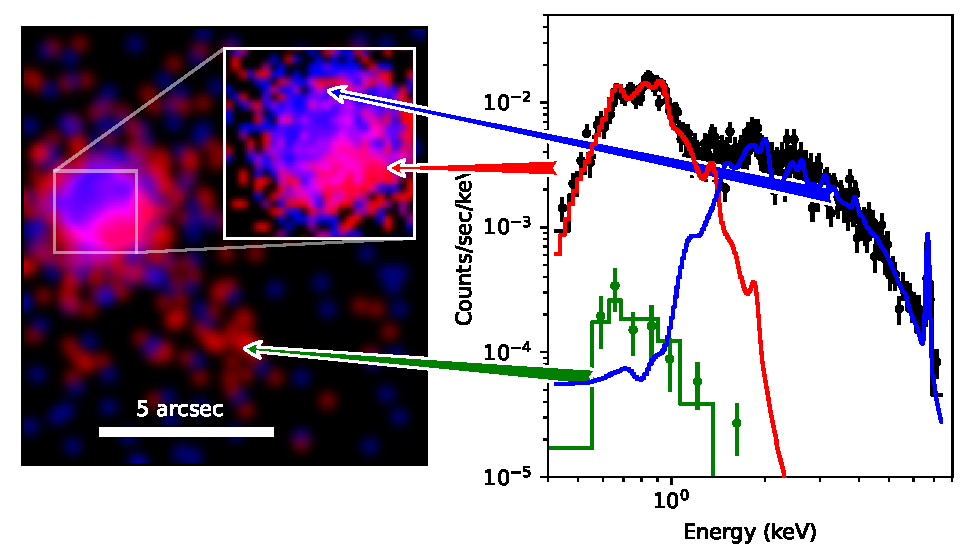
\includegraphics[width=\textwidth]{figs/DGTau.pdf}
\caption{{\bf Left: } Chandra X-ray image of the DG~Tau system. Photons are split in two bands (red: 0.4-1.1~keV, blue: 1.5-6.0~keV). There are three emission components: resolved jet (green arrow) and two components that seem to overlap because of Chandra's PSF: The star itself with hard, coronal emission (blue) and the jet base with soft X-ray emission (red) - see inset for a zoom-in. The main image is smoother and the color stretch is non-linear and chosen for visual clarity.
         {\bf Right: } Spectra from the central source (black) with two components (blue: a hard, highly absorbed, coronal source and a softer, less-absorbed source (red). Green is the faint emission of the resolved jet. Arrows connect spectral components with features in the image. \label{fig:dg_tau_X}}
\end{figure}

\subsubsection{X-rays from the jet base}
The property that sets the X-ray emitting from close to the jet base  ($d\lesssim100\,$au), called Jet Base X-ray emission (JeBaX) in the following, apart from the jets with X-ray emission from the outer jet knots is the  evolution  and not the location of the X-ray emission:
the JeBaX is stationary and no proper motion of individual X-ray emitting knots is seen, as is characteristic for knots in protostellar jets.



JeBaX examples are
HH~154 \citep{Favata_2002,Favata_2006,Schneider_2011,Bonito_2011}, DG Tau \citep[see Fig.~\ref{fig:dg_tau_X};][]{Guedel_2005,Guedel_2008,Schneider_2008}, and HH 540 \citep{Kastner_2005}. RY Tau  may belong to this group, too,  although it's faint jet X-ray emission is seen at more than 140\,au from the star \citep{Skinner_2011}. Also, the so-called two absorber X-ray (TAX) sources belong into this class as their X-ray spectra are composed of a strongly absorbed hard component associated with stellar coronal emission and a weakly absorbed soft component associated with the jet \citep[][]{Guedel_2007}; DG~Tau is also a TAX source with the soft X-ray emission $\lesssim1$\,keV subject to much less absorption than the hard component (see Fig.~\ref{fig:tax}). Flaring in TAX sources affects only the hard and not the soft component, which is further evidence for two different emitting regions being responsible for the soft and hard components \citep{Guedel_2007}; and against a scattering origin of the extended X-ray emission. In the following, we concentrate on DG~Tau and HH~154 here, because 
the observational situation for the other systems is inferior, but we expect that the physical processes leading to the jet's X-ray emission are very similar. In particular, there are no reasons to believe that the spatially unresolved TAX sources differ substantially from DG~Tau.
And although the evolutionary statuses of the different driving sources differ (e.g., L1551~IRS\,5 is often considered a class~I object while DG~Tau is a class~II object), we assume in the following that the mechanisms generating the jet's X-ray emission are very similar in all these systems. We note,  that JeBaX may have a relevant contribution to the ionization of the disk surface inducing disk accretion instabilities \cite{Balbus_1991} and altering the disk chemistry \cite{Glassgold_2004} (TBD:ref).


Figure~\ref{fig:hh154} shows that the spatial distribution of the X-ray emission in HH~154 (also known as the jet from L1551~IRS\,5) is compatible with a source constant in flux and morphology  (\citealt{Schneider_2011}, see also \citealt{Bonito_2011}). The same applies to the  X-ray emission of the DG~Tau jet, where 
\citet{Schneider_2008} performed a careful analysis of the relative astrometry between the soft (jet) and hard (coronal) X-ray emission finding that the (deprojected) spatial offset amounts to about 40\,au in all then available four  Chandra  epochs (see Fig.~\ref{fig:dg_tau_X}), which remains true for all five now available Chandra datasets \citep{Guedel_2011}. 

The spatial extent of the X-ray emission differs between HH~154 and DG~Tau. In
HH~154, X-rays are seen out to about 420\,au with a peak at 140\,au \citep{Schneider_2011} while no significant source extension is seen for the DG~Tau soft comoponent limiting it's size along the jet axis to $\lesssim100\,$au \citep{Schneider_2008}. For HH~154, \citet{Schneider_2011} spatially resolve the spectral properties of the X-ray emission and show that the plasma cools from about 8\,MK to 5\,MK within about 300\,au with a similar trend in all three epochs (2001, 2005, 2009).


The X-ray luminosities are $\sim10^{29}$\,erg\,s$^{-1}$ for both jets with emission measures of $8\times10^{51}\,$cm$^{-3}$ (HH~154) and $3\times10^{52}$\,cm$^{-3}$ (DG Tau), and even though the inner X-ray emission region in DG~Tau is not resolved, we can derive a lower limit for the electron density using some reasonable assumptions for the spatial extent (100\,au in length and a radius of 35\,au) through 
\begin{equation}
n_e \gtrsim \sqrt{\frac{EM}{V}}\,,
\end{equation}
which results in $n_e>10^3\,$cm$^{-3}$  (HH 154) and $>3\times10^3\,$cm$^{-3}$ (DG Tau). At these densities, radiative cooling does not contribute strongly  (see Eq.~\ref{eq:dcool}) and  the expansion of the hot plasma likely dominates the cooling and the X-ray flux reduction \citep{Guedel_2008, Schneider_2011}. 

To explain the JeBaX, one needs a mechanism that constantly (over the decade time scale)  heats the plasma close to the driving source to temperatures resulting in (detectable) X-ray emission ($T\gtrsim3\times10^6$\,K). This plasma then cools while traveling along the jet axis. Such a behavior differs strongly from expectations for an individual plasma blob heated by a strong shock as the resulting, hot post-shock plasma would show some proper motion. Furthermore, the shock heating would need to be very stable always heating the same ``amount'' of plasma to the same temperature. Therefore, a number of different scenarios have been proposed to explain the stationary X-ray emission from protostellar jets.



\subsubsection{Origin of the X-ray emission at the jet base}



In analogy with the X-ray emission at larger distances, shocks have been proposed to cause the X-ray emission at the jet base, too. Due to the location of the JeBaX close to the driving source, shocks  are conceivable that  naturally explain the stationary nature of the X-ray emission. For example, an obstacle in the outflow path, which redirects the flow \citep[either the magnetic field or the dense ambient medium, see][]{Bally_2003,Guenther_2014}, or processes related to jet collimation \citep[e.g.][]{Schneider_2011}. 

A model designed to describe the stationary X-ray emission of HH~154 is a diamond shock forming at the base of the jet, i.e., a shock that forms after a 1\,500\,km\,s$^{-1}$ fast jet with $n=300\,$cm$^{-3}$ exits a 200\,au wide fiducial nozzle potentially representing dense circumstellar material or a magnetic nozzle and rams into a dense ambient medium \citep[$n=3\times10^3\,$cm$^{-3}$,][]{Bonito_2011}. 
Replacing the fiducial nozzle with a magnetic field, \citet{Ustamujic_2016} performed  2.5D MHD numerical simulations for a continuously driven jet ramming into a magnetized medium taking into account magnetic-field oriented thermal conduction  and radiative losses effects. The magnetic nozzle at the jet base leads to the formation of an X-ray emitting stationary shock diamond at its exit  \citep[see 3D reconstruction in left panel in Fig.~\ref{fig:ustamujic} and][]{Ustamujic_2016}. The shock reaches temperatures of few million degrees and densities of $\sim 10^4$cm$^{-3}$ (see left panel in Fig.~\ref{fig:ustamujic}) and is stationary over the time covered by the simulations ($\approx$40-60~yr). 

Later, in \cite{Ustamujic_2018}, they investigated the effect of perturbations in the X-ray emitting stationary shocks described here, and the stability and detectability in X-rays of these shocks, through MHD numerical simulations of pulsed (both light and heavy) jets. They found that, under certain conditions, the quasi-stationary shock formed at the base of the jet continues emitting in X-rays even when perturbations are present (see right panel in Fig.~\ref{fig:ustamujic}, see also \cite{Ustamujic_2018}). Interestingly, in both the light and heavy jet scenarios explored and described with very different physical conditions, they found similar collimation (magnetic) mechanisms forming a quasi-stationary X-ray emitting shock at the base of the jet \cite{Ustamujic_2018}. They also applied their light and heavy models to HH~154 (see right panel in Fig.~\ref{fig:ustamujic}) and DG~Tau, deriving a count rate and synthetic maps in good agreement with X-ray observations (see Figs.~\ref{fig:hh154}~and~\ref{fig:dg_tau_X}).
The feasibility of the stationary-shock scenario at the base of the jet has also been demonstrated through magnetized laser-plasma laboratory experiments.

In contrast to these MHD simulations starting after the jet has been already accelerated,  \citet{Guenther_2014} studied semi-analytically how a fast inner outflow, a stellar wind, interacts with a surrounding, slower disk outflow. The stellar wind initially has a larger opening angle, but is collimated by the magnetic and thermodynamic pressure of the disk wind. \citet{Guenther_2014} show that a stellar wind velocity of 840\,km\,s$^{-1}$, a launch radius of 0.1\,au, and a mass-loss rate of $5\times10^{-10}\,M_\odot$\,yr$^{-1}$ produces X-ray emission with spatial scales and luminosities compatible with observations.

\begin{figure}[t]
    \centering
    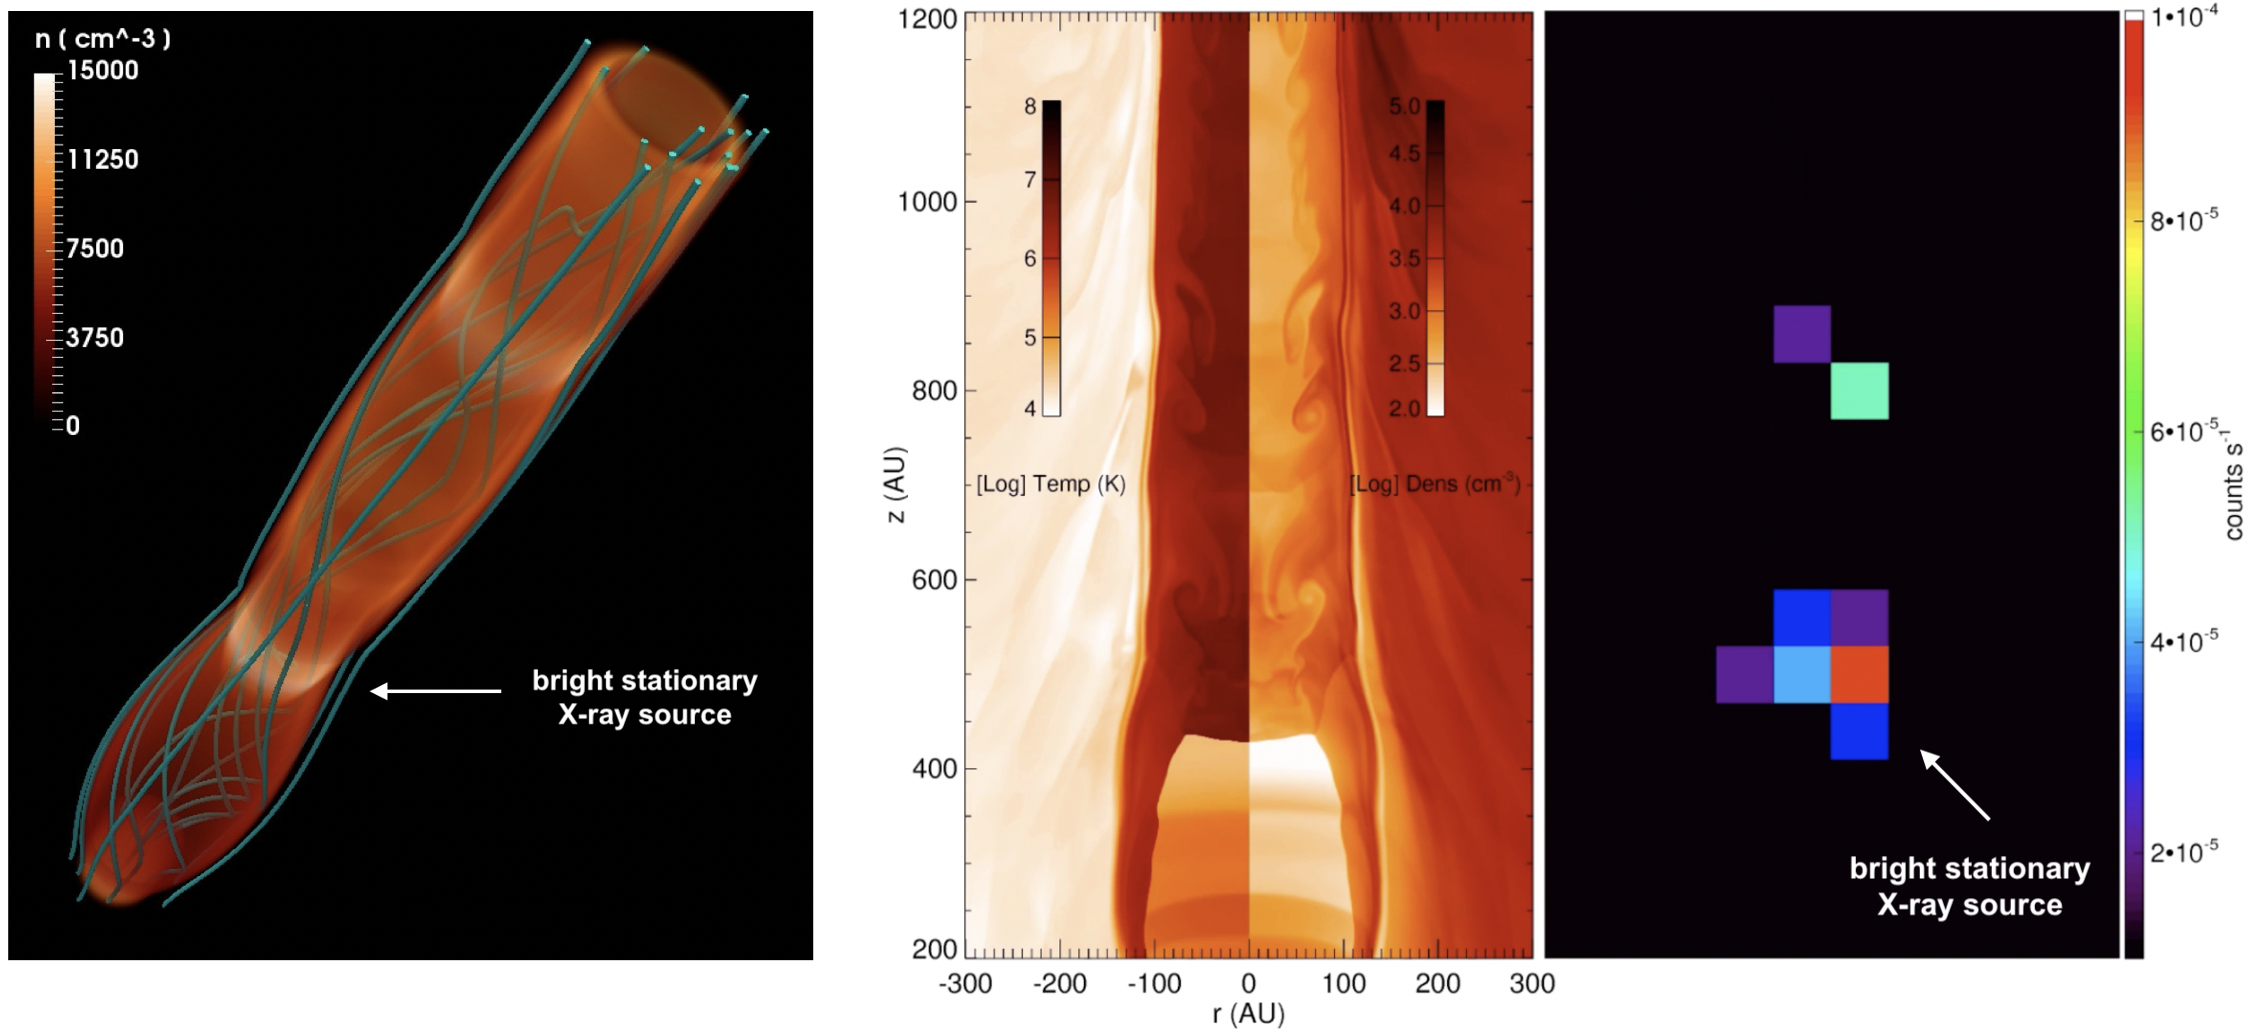
\includegraphics[width=12cm]{figs/ustamujic.png}
    \caption{A combination of Figs. from Ustamujic et al. 2016,2018,2019. I'd rather prefer this one in order to include the X-ray emission synthesized from the model (which is in agreement with the observations).}
    \label{fig:ustamujic}
\end{figure}



All models employing shocks for heating the outflowing plasma to X-ray emitting temperatures require high flow and shock velocities, which are, however, not seen at other wavelengths. Therefore, \citet{Guedel_2007} and \citet{Schneider_2013a} mention that the jet's magnetic field may contribute to the heating of the jet, e.g., current dissipation and reconnection events. This idea was studied in detail by  \citet{Takasao_2017}. In their model, 
the disk atmosphere is magnetically heated similar to the nanoflare model for the heating of the Sun's corona, i.e., magnetic buoyancy will lead to magnetic loops rising to larger heights in the inner disk where energy is released in reconnection events. Disk magnetic field of 1\,G may be sufficient to produce the observed X-ray luminosity and temperature. In their model, the jet base is the X-ray brightest and cooling by radiation and expansion may be sufficiently suppressed to even produce X-rays at some distance to the launch region. Similar to all other models, the flow velocity likely exceeds 300\,km\,s$^{-1}$ even without requiring shocks to provide the thermal energy as cooling would lower the outflow's X-ray emission too strongly already close to the source incompatible with observations.

\subsubsection{Comparison with other jet tracers}
How does the X-ray emission compare with data at other wavelengths? First, 
evidence for stationary structures also exists in tracers of lower temperature plasma, e.g., [Fe~{\sc ii}]~1.644\,$\mu$m  \citep{White_2014} and [O~{\sc i}]~$\lambda6300$ data \citep[][]{Schneider_2013a}, neither of which is clearly downstream of the X-ray emission. 

Second, optical and NIR jet observations suggest shock velocities of only 30--100\,km\,s$^{-1}$ close to the source \citep[e.g., ][]{Lavalley_2000, Hartigan_2007}. The detection of [O~{\sc iii}]~$\lambda5007$ emission in some shocks may imply temperatures of $\log~T\sim5$ although the bulk emission still appears to result from lower temperature plasma \citep[e.g.,][]{Bacciotti_2011,Nisini_2016}. On the other hand, the shock velocity appears to increase with post-shock velocity and there is evidence for high-velocity ($\sim400\,$km\,s$^{-1}$) material close to the star in some sources from absorption studies, e.g., sub-continuum absorption in He~{\sc i}\,$\lambda10830$ \citep[e.g.][]{Edwards_2006} or FUV lines like C~{\sc ii} \citep{Xu_2021}, i.e., flow velocities in excess of 400\,km\,s$^{-1}$. However, typical velocities are slower and even flow velocities of 400\,km\,s$^{-1}$ would still require a stationary obstacle for shock velocities sufficiently fast for X-ray emission. 

Third, observations of emission tracing the temperature range intermediate between the ``classical''  and the X-ray emitting jet have been obtained with HST (C~{\sc iv}, [Ne~{\sc iii}]). \citet{Schneider_2013a} and \citet{Skinner_2018} obtained long-split HST C~{\sc iv} data of the DG~Tau and RY~Tau  jets. In both jets, the C~{\sc iv} is located close to the star; the C~{\sc iv} emission in the DG Tau jet is concentrated in a discrete structure overlapping with the X-ray centroid ($\approx0.2$\,arcsec)  while 
the C~{\sc iv} flux monotonically decreases away from the source in RY~Tau. In both jets, the deprojected C~{\sc iv} velocities decrease from about 300\,km\,s$^{-1}$ close to the star to roughly 200\,km\,s$^{-1}$, which is faster than the optical emission in both jets.

Highly ionized plasma is also traced by [Ne~{\sc iii}]~$\lambda3869$ emission\footnote{A shock velocity of $\gtrsim100\,$km\,s$^{-1}$ is required to produce [Ne~{\sc iii}] in shocks.} in the Sz~102 jet \citep{Liu_2021}. The [Ne~{\sc iii}] emission is spatially extended along the jet axis, and smoothly decreases in flux away from the star, like the C~{\sc iv} emission in RY~Tau. Therefore, \citet{Liu_2021} prefer a scenario in which the high ionization is produced very close to the star, likely due to X-ray irradiatoin,  and remains frozen in the jet as the recombination time scale appears compatible with the spatial extend of the [Ne~{\sc iii}] emission and the measured flow velocity of 250--300\,km\,s$^{-1}$.

Fourth, mass-loss rates estimated for the $10^5$\,K jets ($\sim10^{-9}\,M_\odot$\,yr$^{-1}$) may be regarded as intermediate between the ``classical'' \citep[$\sim10^{-8}\,M_\odot$\,yr$^{-1}$][]{} and X-ray emitting jets ($\dot{M}_{out}(\textrm{X-ray})\sim10^{-10}\,M_\odot$\,yr$^{-1}$, see above). 


In summary, a viable scenario for the X-ray emission may be based on the innermost, fastest part of the jet, which also experiences the strongest heating while carrying only a fraction of the mass-loss. In this picture, the X-ray and C~{\sc iv} emission would represent the inner and fastest components of the onion-like structure of protostellar jets extending the regularly detected low-, medium-, and high-velocity components to even higher velocities and temperatures. One or a number of discrete shocks sufficiently fast for the X-ray emission appear challenging to realize, because measured flow velocities are on the low end of the shock velocity range required to produce the X-ray emission. This  may be circumvented by assuming that (a) velocities are post-shock velocities with much higher initial flow velocities and (b) that only a fraction of the flow participates in the X-ray production. Therefore, other mechanisms like magnetic heating may be required to explain the high temperatures at velocities only slightly larger than ``classical'' jet where shock velocities fall short of the ones required for the X-ray emission by almost a factor of ten. Additional observations and simulations are needed to investigate the interplay between the different temperature components in protostellar jets, which will potentially also constrain the magnetic field in the jet launching region.



% \begin{figure}
%     \centering
%     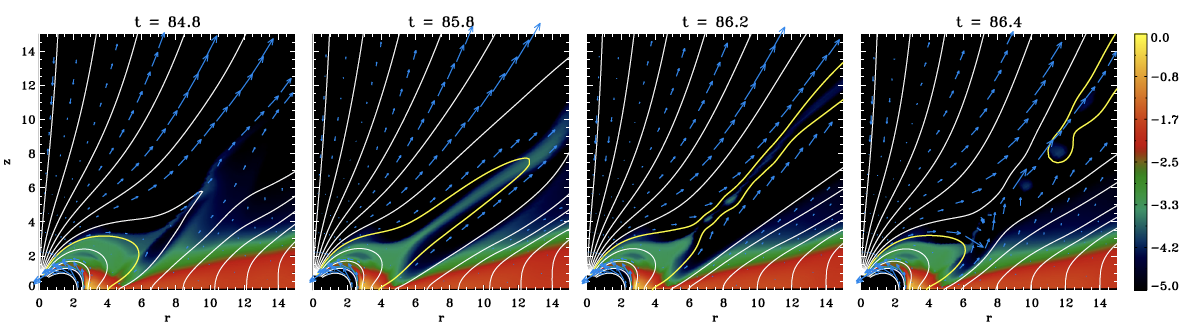
\includegraphics[width=12cm]{figs/Zanni2013.png}
%     \caption{Temporal evolution of the periodic inflation/reconnection process which characterizes the dynamics of the magnetospheric ejections. Need to ask for permission.}
%     \label{fig:zanni2013}
% \end{figure}


% \begin{figure}
%   \centering
%    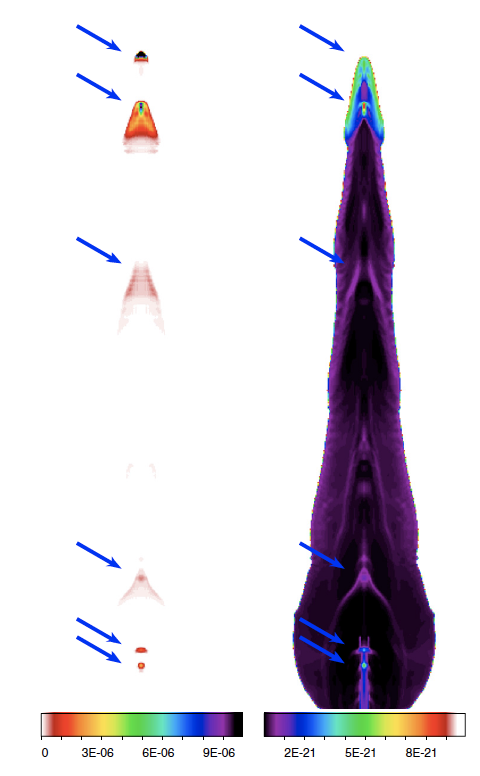
\includegraphics[width=0.8\textwidth]{figs/Bonito2010b.png}
%    \caption{X-ray emission from HH objects \cite{Bonito_2010b}. Need for permission. \label{fig:Bonito2010b}}
% \end{figure}
% % 
% 
% \subsubsection{Mass loss rate}
% 
% \cite{Watson_2016}: Outflow activity associated with all stages of early stellar evolution from Class 0 to Class II. General trend: decrease of mass outflow and mass accretion rates with increasing age while maintaining rough proportionality (Fig. 7, \cite{Watson_2016}). Also increasing mass outflow rate with luminosity; the power seems to decrease with age (Fig. 6, \cite{Watson_2016}).
% 
% \begin{figure}
%   \centering
%    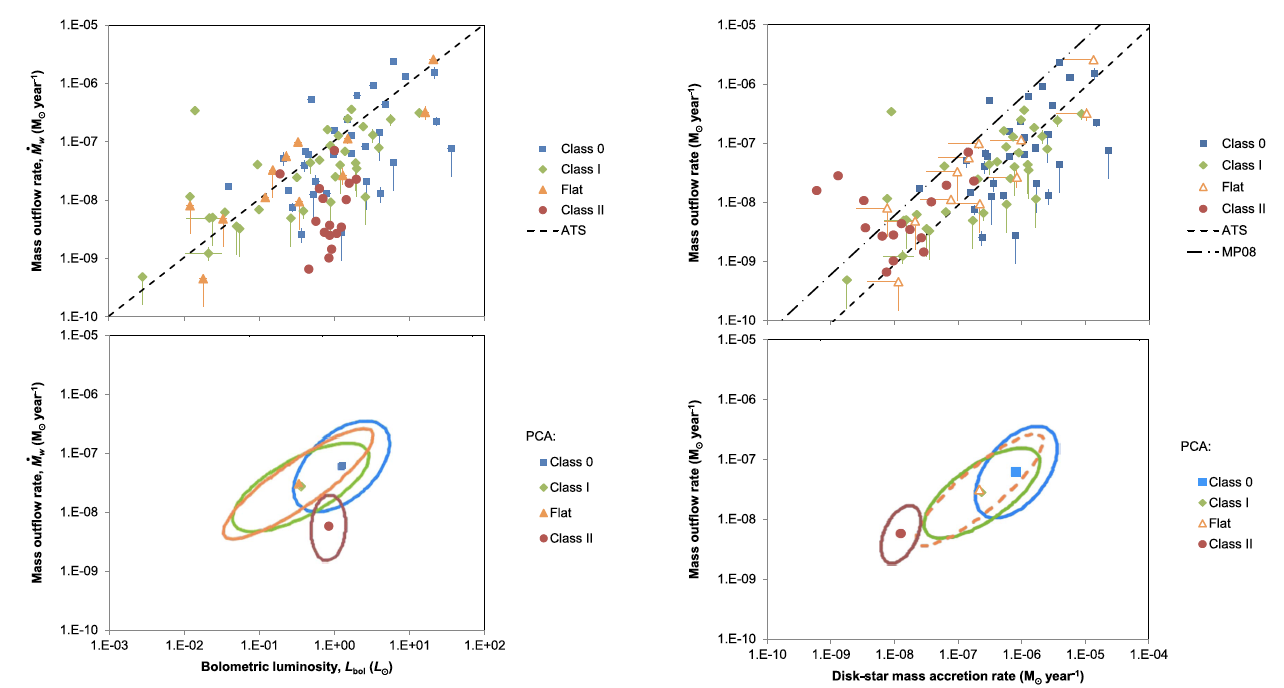
\includegraphics[width=1.0\textwidth]{figs/Watson2016}
%    \caption{Figure here? Outflow activity from \cite{Watson_2016}. Need for permission. \label{fig:watson2016}}
% \end{figure}


